\chapter{Review of the state of the art}

\section{Evolution in internal combustion engines technology and efficiency}

In this section a review of the key technical improvements occurred to internal combustion engines in the last decades is presented, among with a brief explanation of the current emission limitation rules for both the USA and Europe. The final section will cover the importance of \emph{Waste Heat Recovery} (WHR) and why it needs to be researched and adopted in the next years in order to achieve the planned emissions limitation objectives.

\subsection{Improvements on overall engine efficiency in the last decades}

Since the petroleum crysis of the '70s, an increasing effort on reduction of fuel consumption and increase of power density has begun.

\begin{figure}[ht]
  \centering
  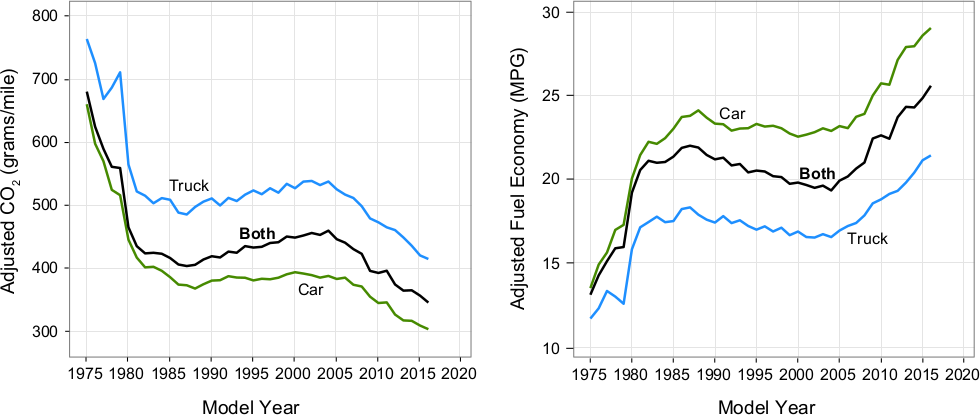
\includegraphics[width=\textwidth]{figures/review/adj_fuel_economy.pdf}
  \caption{Adjusted CO\textsubscript{2} and fuel economy for vehicles model year from 1975 to 2016\label{fig:adj_fuel_economy} }
\end{figure}

As shown in Figure~\ref{fig:adj_fuel_economy}~\cite{EPA2016}, during the last four decades, the fuel consumption and carbon dioxide emissions has been vastly reduced. This great improvement has been possible thanks to some key technical turning points.

One of the main design aspects that have changed significantly over time is how the fuel is delivered into the engine. Until the early 1980s the majority of engines used carburetors to meter fuel delivered to the combustion chamber. More recently, engines with gasoline direct injection (GDI) have begun to replace engines with port fuel injection. GDI equipped engines were first introduced with very limited production in Model Year (MY) 2007. Eight years later GDI engines were installed in about 42\% of MY 2015 vehicles, and are projected to achieve a 49\% market share in MY 2016~\cite{EPA2016}.

Another key aspect of engine design that has been vastly improved is the valve-train. The number of valves per cylinder and the ability to alter valve timing during the combustion cycle allowed significant power and efficiency improvements, as nowadays almost the entire fleet of the most relevant car manufacturers has converted to multi-valve design. While some three and five valve engines have been produced, the vast majority of multi-valve engines are based on four valves per cylinder~\cite{EPA2016}. In addition to the number of valves per cylinder, designs have evolved that allow engine valves to vary the timing when they are opened or closed with respect to the combustion cycle, creating more flexibility to control engine efficiency, power, and emissions. In Figure~\ref{fig:improvement_valve_fuel_delivery}, the fuel consumption reduction made possible by the improved valve-train and fuel delivery is shown. 

\begin{figure}[ht]
  \centering
  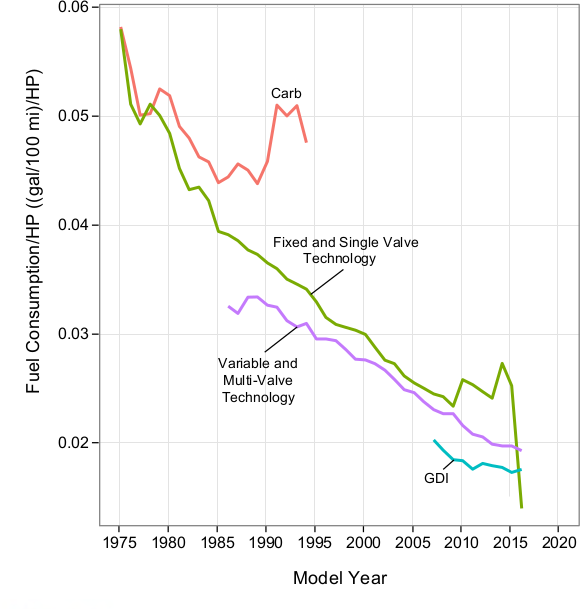
\includegraphics[width=0.7\textwidth]{figures/review/improvement_valve_fuel_delivery.pdf}
  \caption{Trends of fuel consumption variation with the introduction of major fuel delivery and valve-train control technologies \label{fig:improvement_valve_fuel_delivery} }
\end{figure}

As a result of the new fuel delivery systems, along with other reasons, two very noticeable trends in horsepower and displacement delineated. Average horsepower climbed consistently from MY 1982 to MY 2008. Since MY 2008, horsepower trends have been less consistent, and may be beginning to flatten out. From MY 1975 to 1987, the average engine displacement of new vehicles dropped dramatically by nearly 40 \%. From MY 1988 to 2004, displacement generally grew slowly, but the trend reversed in 2005 and engine displacement has been generally decreasing since. In MY 2016, engine displacement is projected to reach the lowest point on record, below the previous lowest average displacement reached in MY 1987~\cite{EPA2016}.

The contrasting trends in horsepower increase and displacement decrease are a proof of the continued improvements in engine design and of the impact of new technologies. The final result is a steady quasi-linear increase of the power density from around 0.5~$\frac{HP}{Displacement}$ in 1975 to around 1.4~$\frac{HP}{Displacement}$ in 2016, with a growth rate of 0.02~$\frac{HP}{in^{2} \cdot year}$. Also the average number of cylinders has gradually reduced.

In Figure~\ref{fig:technology_trends}, a summary of the time trends of the major innovations is reported.

\begin{figure}[ht]
  \centering  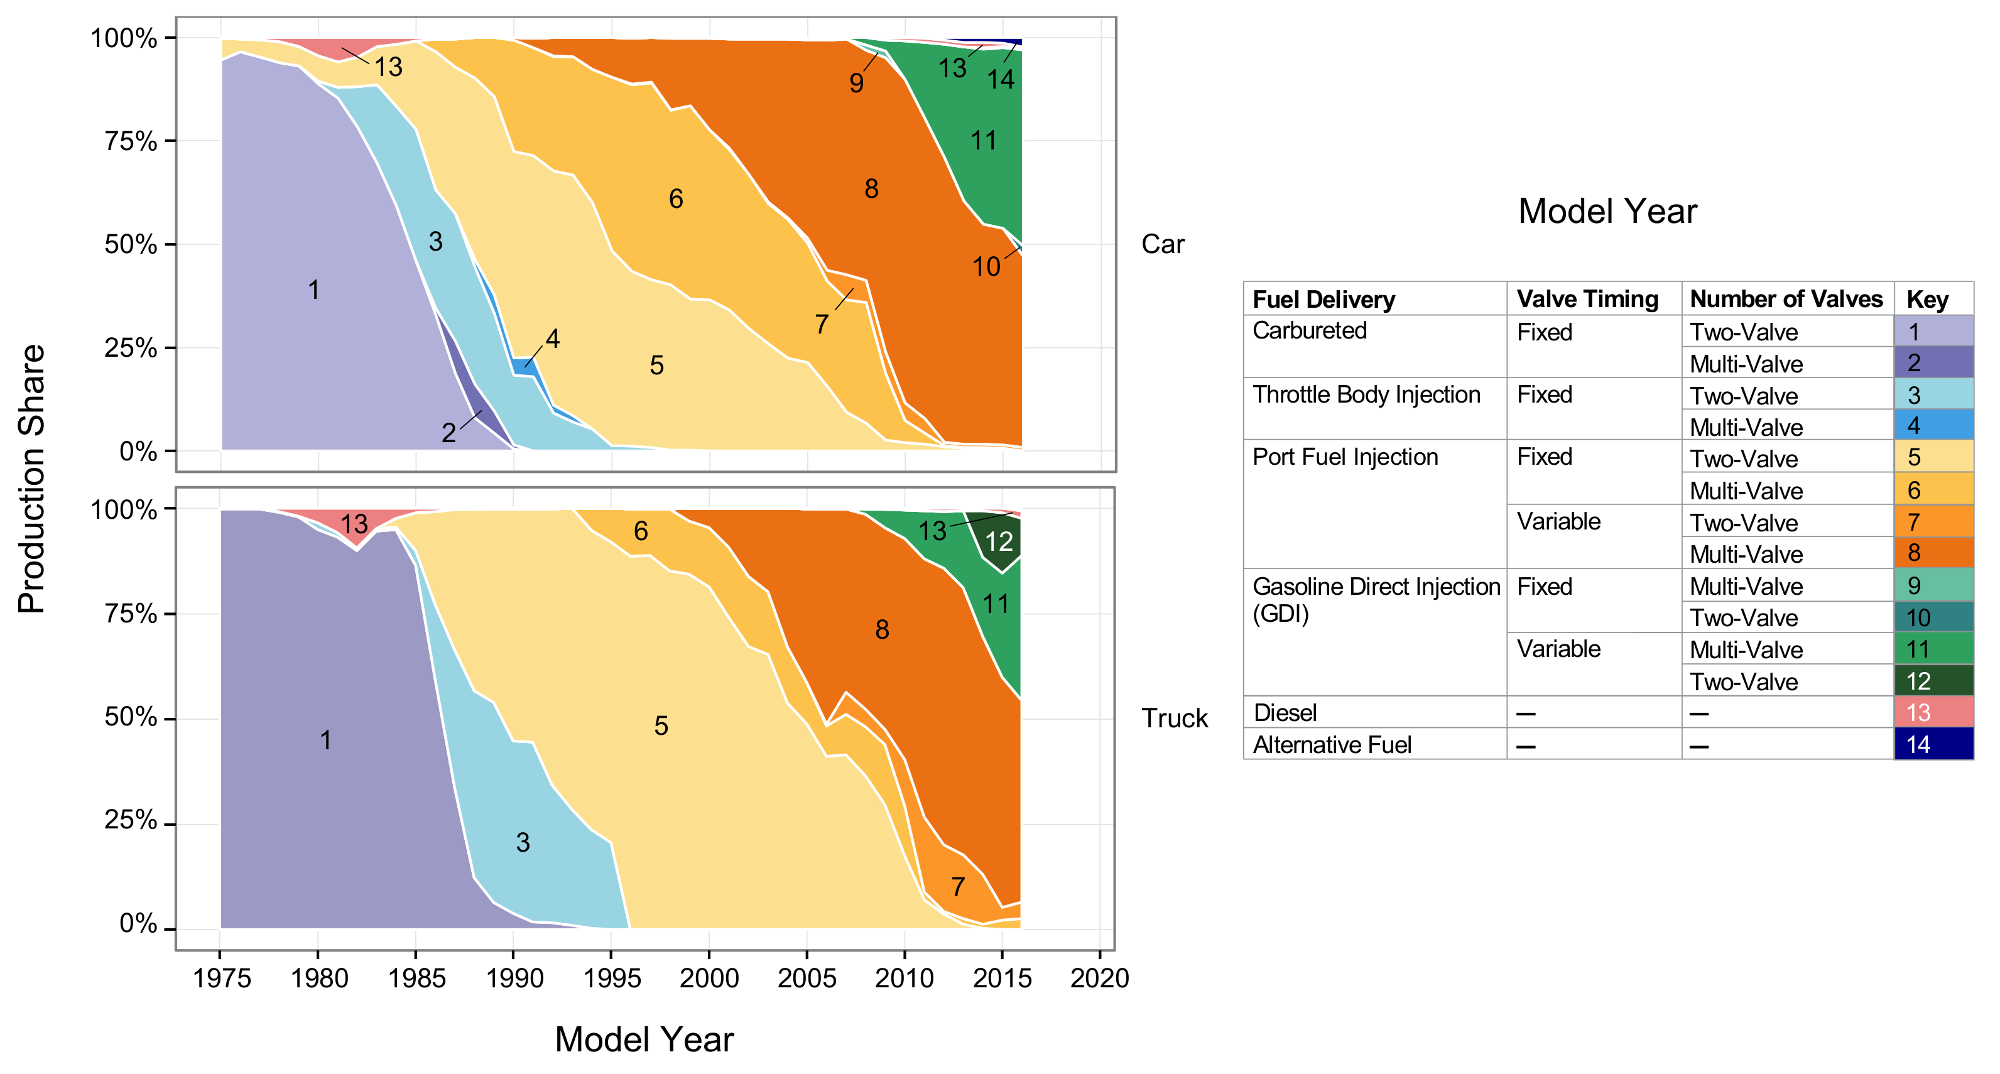
\includegraphics[width=\textwidth]{figures/review/technology_trends.png}
  \caption{Percentage of MY equipped with a certain technology  \label{fig:technology_trends} }
\end{figure}


\subsection{Emission limitations and trends in nowadays technology improvement}
\label{sec:technology_improvements}

Emission limitations are among the main drivers that fostered the continuous strive of greater efficiency in internal combustion engines. In Figure~\ref{fig:emission_standards} a review of the most important emissions standards from across the world, and their Euro equivalence is presented~\cite{Miller2014}. In Figure~\ref{fig:emission_levels} are reported the emission limits for gasoline and diesel powered light vehicles in both USA and Europe~\cite{Transportpolicy.net2016}.

\begin{figure}[ht]
  \centering
  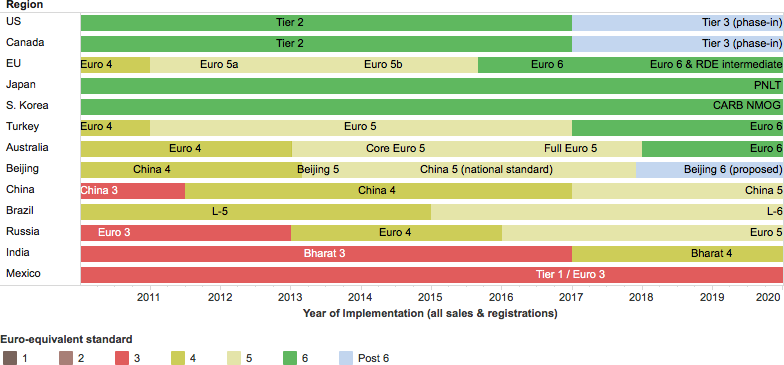
\includegraphics[width=\textwidth]{figures/review/emission_standards.png}
  \caption{Comparison of emissions standards with reference to Euro standards\label{fig:emission_standards} }
\end{figure}

\begin{figure}[ht]
  \centering
  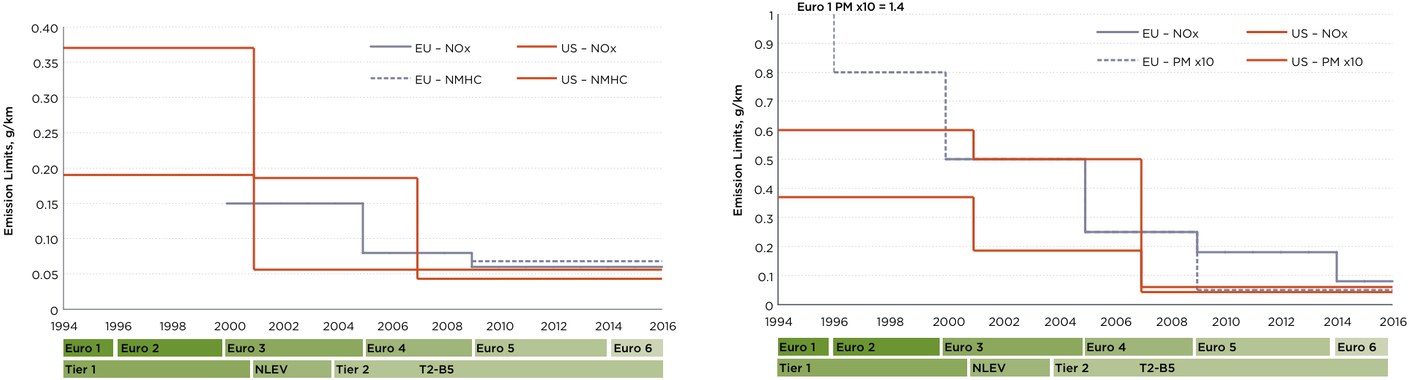
\includegraphics[width=\textwidth]{figures/review/emissions_levels.png}
  \caption{Emissions limits for a) Gasoline and b) Diesel light vehicles in USA and Europe\label{fig:emission_levels} }
\end{figure}

In order to respect the emission standards imposed by current and future rules, the major car manufacturers are adopting new technologies, and some trends are delineating. 

Probably the most noticeable trend in new engines is the \emph{turbo-downsizing}. This new group of engines is characterized usually by a similar power output with respect to the engine that are replacing, but a smaller displacement. This result is achieved by the introduction of turbochargers and, often but not always, GDI. Turbo downsized engines are an approach to engine design that provides increased fuel economy by using a smaller engine for most vehicle operation, while retaining the ability to provide more power via the turbocharger, when needed. Turbocharged engines are projected to constitute 22\% of new vehicle production in 2016, and the penetration trend appears to increase rapidly~\cite{EPA2016}. This is due to the fact the traditionally turbocharged engines were mainly used in high performance vehicles, while now they are being used also on mainstream vehicles. The increased power density and torque made available by the adoption of the turbocharger allows the shifting to designs with fewer cylingers, while the combination with GDI allows a more efficient engine operation and increases the resistance to knocking. In MY 2016, more than 90\% of new vehicles with gasoline turbocharged engines also use GDI~\cite{EPA2016}. In Figure~\ref{fig:turbodownsizing_distribution}, the distribution of gasoline turbo vehicles is shown. Other new technologies that are gaining traction in the engine design environment are Cylinder Deactivation, Non-Hybrid Stop/Start, and more advanced transmissions, both in form of transmissions with seven or more gears or Continuous-Variable Transmissions (CVT).

\begin{figure}[ht]
  \centering
  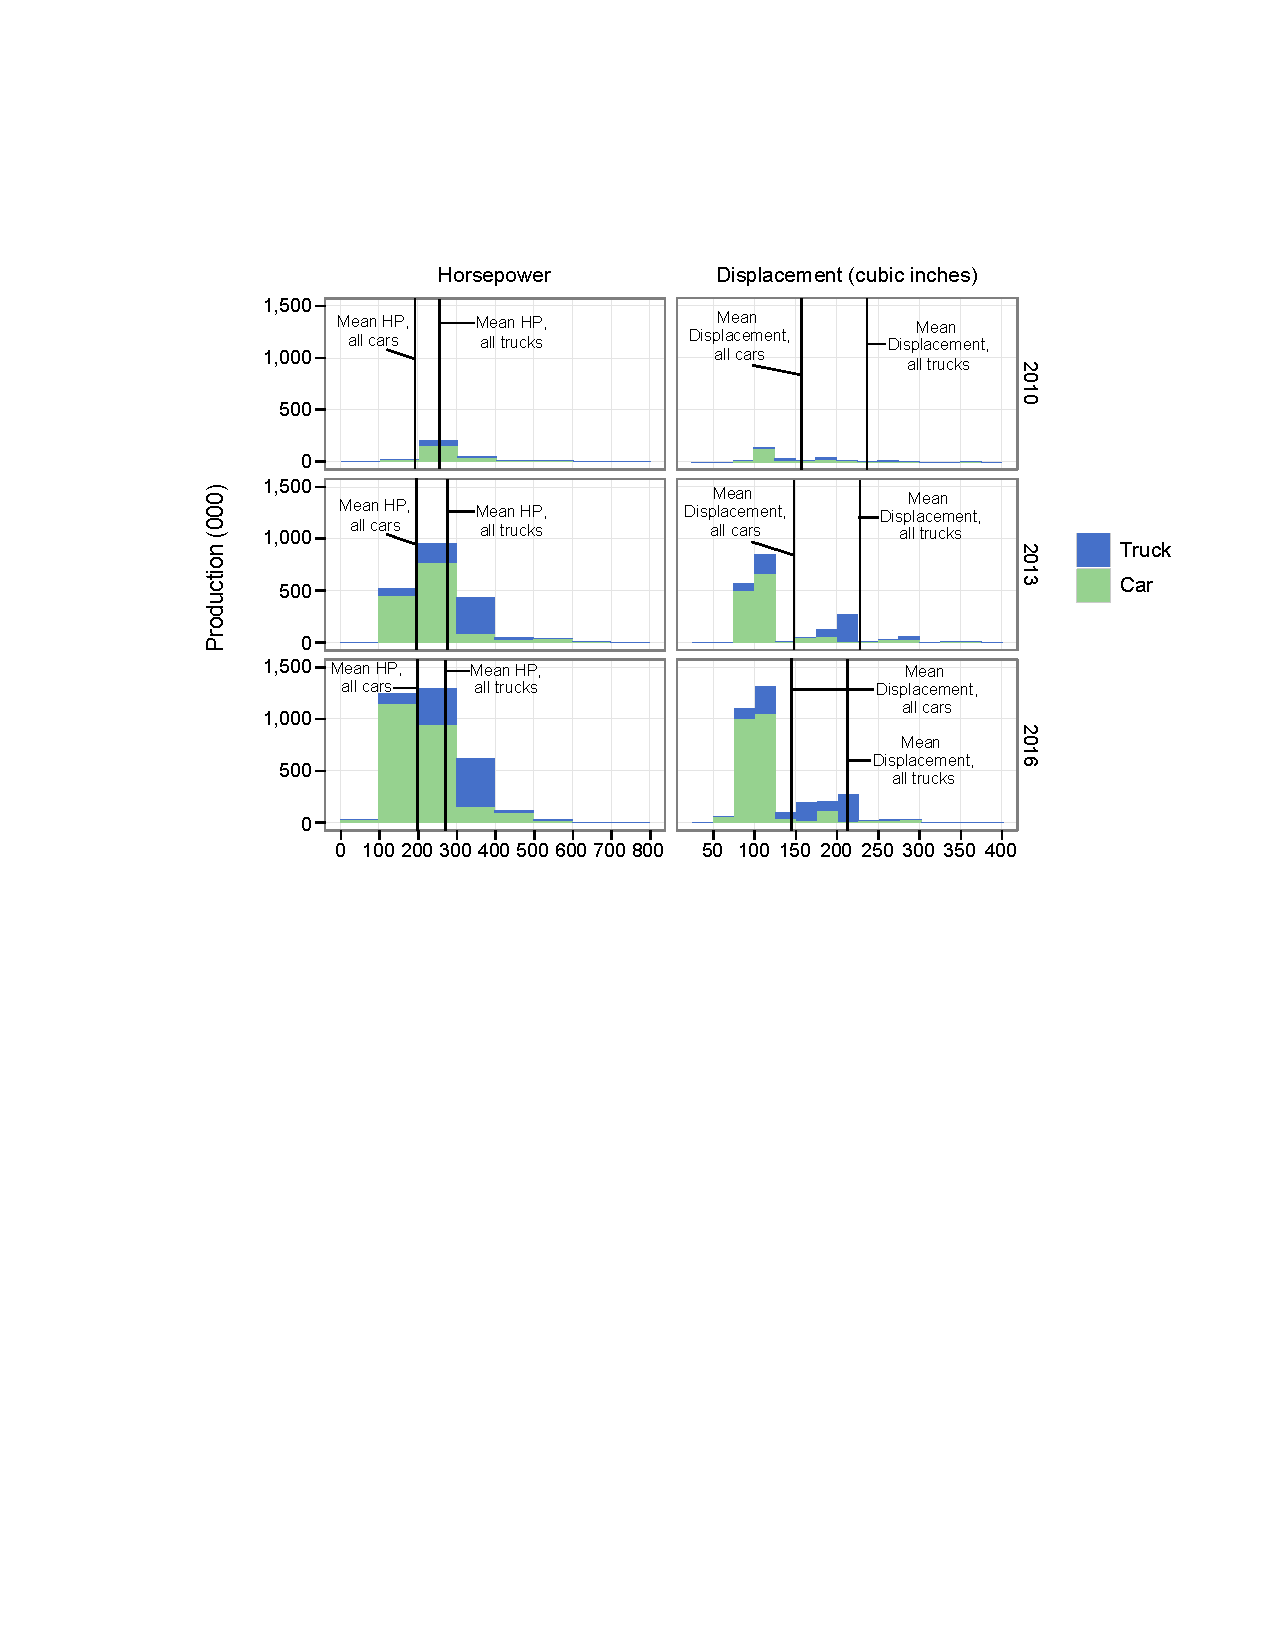
\includegraphics[width=0.8\textwidth]{figures/review/turbodownsizing_distribution.pdf}
  \caption{Distribution of Gasoline Turbo Vehicles by Displacement and Horsepower, MY 2010, 2013, and 2016\label{fig:turbodownsizing_distribution} }
\end{figure}



\emph{Hybrid} vehicle technology is the most diffused technique used to increase the fuel efficiency in ways that transcend the pure ICE efficiency increase. Hybrid vehicles utilize larger battery packs, electric motors, and other components that can  increase vehicle fuel economy. Benefits of hybrids include:
\begin{itemize}
\item regenerative braking which can capture energy that is otherwise lost in conventional friction braking to charge the battery
\item availability of two sources of on-board power which can allow the engine to be operated at or  near its peak efficiency more often
\item shutting off the engine at idle.
\end{itemize} 

Most hybrids provide higher fuel economy than comparable vehicles, although some hybrids have been offered as more performance-oriented vehicles with more minor fuel economy improvements. In Figure~\ref{fig:hybrids} it's shown the distribution in time of the fuel economy between hybrid and non hybrid vehicles, and the historical production of hybrid and electric vehicles.

\begin{figure}[ht]
  \centering
  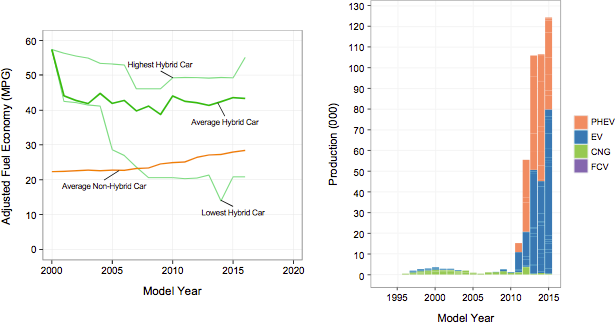
\includegraphics[width=\textwidth]{figures/review/hybrid.png}
  \caption{Comparison fuel economy between non hybrid and hybrid cars and hybrid cars production \label{fig:hybrids} }
\end{figure}


While the average fuel economy of hybrid cars remains higher than the average fuel economy  of non-hybrid cars, the difference appears to be narrowing. Average hybrid car fuel economy  has been relatively stable since MY 2001, while the fuel economy of the average non-hybrid car has increased more than 27\%. Since MY 2004, the difference in fuel economy between the average hybrid midsize car and the average non-hybrid midsize gasoline car has narrowed from about 25 mpg to about 14 mpg. The primary reason for this trend is continued improvements to the internal combustion engine. Additionally, many technologies introduced or emphasized in early hybrids, such as improved aerodynamics, low rolling resistance tires, and increased use of lightweight materials, have also become more common on non-hybrid vehicles~\cite{EPA2016}.

\subsection{The importance of waste heat recovery}

In the previous sections a brief review of how some of the key technical improvements have modified engine design, performances and fuel consumption have been provided.

One of the main causes of the relatively low efficiency of even modern ICEs is that a significant amount of energy produced by fuel combustion is wasted in form of heat, then not used to produce useful power. In internal combustion engines, only a small part of the fuel energy flow is transformed into power available at the crankshaft. For the best points of operation, diesel engines have a maximum efficiency approaching 45\% while gasoline engines have efficiencies of about 35\%. For both engines, the most part of the fuel energy flow is therefore lost as coolant heat flow and exhaust gases heat flow. In everyday operating conditions, cars have average engine efficiencies on driving cycles well below their top values, with the heat flow lost in the exhaust gases and the engine coolant increasing accordingly. In many driving conditions, the waste heat flow represents an important part of the fuel energy flow. The energy flow potentially available to be converted to usable power in the exhaust gases and the coolant is therefore quite significant~\cite{Boretti2012}. Considering the large number of vehicles in the world, such waste energy makes great impact to our environment globally.

It has been estimated that the thermal efficiency of a modern IC engine is limited to 20 - 40\% while 33\% of the fuel energy from a typical medium-size passenger vehicle is carried away by exhaust gases and 29\% is carried away by engine cooling water in urban traffic conditions. Depending on engine type and operating conditions, the IC exhaust gas temperature usually varies from 500 to \SI{900}{\celsius} and engine cooling water temperature is around \SI{100}{\celsius}. It is reported that for a typical light duty 4 cylinder spark ignition engine, the waste energy carried by the exhaust gas ranges from 4.6 to 120 kW and cooling water heat ranges from 9 to 48 kW \cite{ElChammas2005}, which makes the exhaust gas and engine cooling heat very attractive for energy recovery. It's possible to harvest part of this waste energy from vehicles and produce regenerated mechanical or electrical power.

According to \cite{Conklin2010}, experimental data coming from a series of tests on a turbo-charged 2007 Saab vehicle shows engine-out exhaust temperature from 400 to \SI{600}{\celsius}. The exhaust temperature range of naturally aspirated gasoline engine is higher, typically from 450 to \SI{800}{\celsius}. The same research performed a FTP-75 test cycle with the aforementioned vehicle, and measured that the total fuel energy consumed during the course of the driving cycle is approximately 58.5 MJ, or about 1.7 L of unleaded gasoline fuel. The percentage of fuel energy converted to useful work for this driving cycle (i.e. the vehicle thermal efficiency) is 10.4\%. A much larger portion of fuel energy, 27.7\%, exits the vehicle in the form of thermal energy in the exhaust, while the remaining 61.9\% of the energy balance consists of energy losses to friction, coolant, and other. Only a portion of the energy in the exhaust is available for recovery due to process irreversibilities, ambient conditions, or other.

% BEGIN RECEIVE ORGTBL first_second_law
\begin{table}
  \begin{center}
    \begin{tabular}{lrr}
      & 1st law & 2nd law \\
      \hline
      Brake work & 10.4\% & 9.7\% \\
      Exhaust & 27.7\% & 8.4\% \\
      Irreversibilities, Friction, Coolant, and other & 61.9\% & 81.9\% \\
    \end{tabular}
    % % END RECEIVE ORGTBL first_second_law
    % \begin{comment}
    %   #+ORGTBL: SEND first_second_law orgtbl-to-latex
    %   |                                                 | 1st law | 2nd law |
    %   |-------------------------------------------------+---------+---------|
    %   | Brake work                                      |   10.4% |    9.7% |
    %   | Exhaust                                         |   27.7% |    8.4% |
    %   | Irreversibilities, Friction, Coolant, and other |   61.9% |   81.9% |
    % \end{comment}
    \caption{1\textsuperscript{st} and 2\textsuperscript{nd} law of thermodynamics fuel energy and exergy distributions}
    \label{table:1st_2nd_law}
  \end{center}
\end{table}

In Table~\ref{table:1st_2nd_law} are reported the energy and exergy distributions with respect of the fuel entering the engine. It's possible to notice how, according to the 2\textsuperscript{nd} law of thermodynamics, the exhaust exergy is nearly as high as the amount of brake work. Thus, there is an abundant amount of available energy present in the exhaust of modern gasoline vehicles that can be used to improve overall system efficiency if an effective means of energy recovery can be employed. In another research \cite{Dolz2012}  the value of exhaust gases mentioned to be 18.6\% of total combustion energy. It is also found that by installing heat exchanger to recover exhaust energy of the engine could be saved up to 34\% of fuel saving \cite{Wang2013}.

Many studies highlighted the validity of the idea of recovering this waste heat to produce additional power, and the research and actual production efforts showed promising results. In Table~\ref{Table:ORC_research_list} are listed some of the most relevant research and production vehicles equipped with a waste heat recovery system, among with the achieved increase in thermal and mechanical efficiency.

\begin{table}[]
  \centering
  \resizebox{\textwidth}{!}{
    \begin{tabular}{lllllll}
      \hline
      Reference                        & Year & Vehicle       & Heat Source                 & Research method & $\Delta\eta_{th}$ & $\Delta\eta_{mec}$ \\ \hline
      \cite{Oomori1993b}               & 1993 & Passenger car & Coolant                     & Experiment      & /                 & 3\%                \\
      \cite{ElChammas2005}             & 2005 & HEV           & Exhaust                     & Numerical       & 1.3-5\%           & /                  \\
      \cite{Arias2006}                 & 2006 & Prius         & Exhaust + engine block      & Numerical       & 5.50\%            & /                  \\
      \cite{Endo2007, Kadota2008}      & 2007 & HEV           & Exhaust                     & Experiment      & 3.80\%            & /                  \\
      \cite{Freymann2008}              & 2008 & 3 series      & Exhaust + Coolant           & Experiment      & 5.70\%            & /                  \\
      \cite{Duparchy2009}              & 2009 & HEV-Prius     & Exhaust + Coolant           & Numerical       & /                 & 9\%                \\
      \cite{He2011, ZHANG2011}         & 2011 & Toyota 8A-FE  & Exhaust, Lubricant, Coolant & Experiment      & 12-17.3\%         & /                  \\
      \cite{Freymann2012, Horsta}      & 2012 & 5 series      & Exhaust                     & Experiment      & /                 & 6\%                \\
      \cite{Boretti2012, Boretti2012a} & 2012 & 1.8L engine   & Exhaust + Coolant           & Numerical       & 1.7-5.1\%         & /                  \\
      \cite{Wang2016a}                 & 2012 & BL18T engine  & Exhaust + Coolant           & Numerical       & 3-6\%             & /                  \\
      \cite{Domingues2012}             & 2013 & 2.8L VR6      & Exhaust                     & Experiment      & /                 & 2.64-6.96\%        \\ \hline
    \end{tabular}}
  \caption{Research results on waste heat recovery benefits}
  \label{Table:ORC_research_list}
\end{table}

\section{Introduction to bottoming recuperative cycles}

A bottoming cycle is a waste-heat recovery thermodynamic cycle that recaptures the unused energy and uses it to produce steam to drive a steam turbine generator to produce additional energy. In Figure~\ref{fig:bottoming} is shown a general configuration for a bottoming cycle. In the passenger case car, the thermal process upstream the cycle is the internal combustion engine itself.

\begin{figure}[ht]
  \centering
  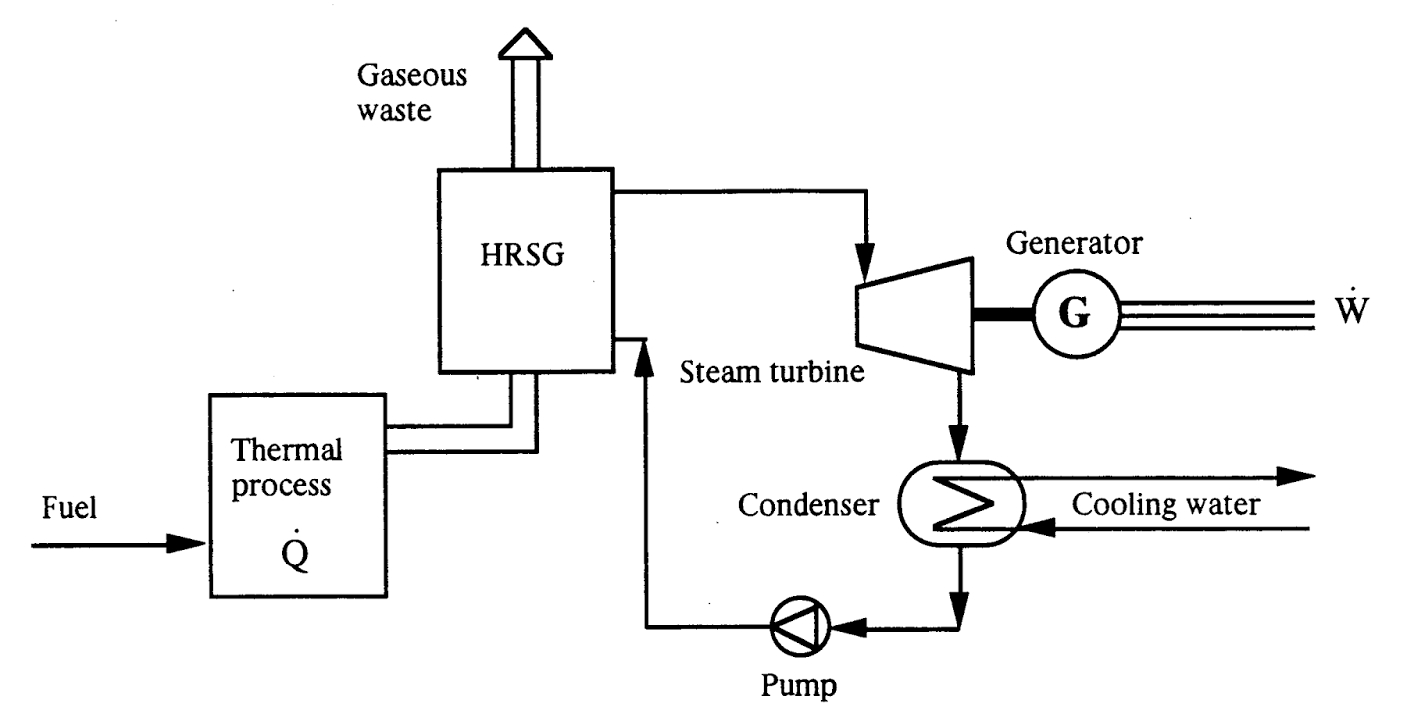
\includegraphics[width=0.7\textwidth]{figures/review/bottoming.jpg}
  \caption{Bottoming cycle \label{fig:bottoming} }
\end{figure}
~

A bottoming cycle is a powerful mean to recover the waste heat produced by an automotive internal combustion engine, and the additional power produced can be employed in different ways. It is possible to produce additional mechanical work, increasing the torque at the shaft, or produce electrical work that can be employed in different ways. Usually the selected recovery strategy is to use the recuperative cycle to produce mechanical power: this implementation is simpler and effective, but fails to achieve the maximum potential with respect to the operative conditions of the additional cycle. In this configuration the angular speed of the turbine is the same as the one of the shaft, but this speed can be different from the one of maximum efficiency of the turbo-machine.

The configuration that converts the additional power in electrical power can solve this issue. Being the system no more coupled with the shaft of the internal combustion engine but with an electric generator, the rotational speed of the turbine can be varied at will in order to achieve the most efficient operative point. The electricity produced can be stored in batteries is they are available (i.e. Hybrid or Plug-in vehicle), or used to power up auxiliaries and reduce the alternator load on the engine.

In the following sections a brief overview of the most common thermodynamic cycles that can be used as a recuperative bottoming cycle will be provided.

\subsection{Steam Rankine cycle}

The steam Rankine cycle is one of the most famous and used thermodynamic cycles for producing power. In this cycle the heat is provided externally to a closed loop, in which water flows as a working fluid. The efficiency of the Rankine cycle can be calculated as:

\begin{equation} \label{eq:eta_rankine}
  \eta_t = \frac{\dot{W}_{thermal}-\dot{W}}{\dot{Q}_{in}} \approx \frac{\dot{W}_{turb}}{\dot{Q}_{in}}
\end{equation}

This type of cycle is commonly used in thermal power generation plants. The efficiency of the Rankine cycle is limited by the high heat of vaporization of the working fluid. Also, unless the pressure and temperature reach super critical levels in the steam boiler, the temperature range the cycle can operate over is quite small: steam turbine entry temperatures are typically around \SI{565}{\celsius} and steam condenser temperatures are around \SI{30}{\celsius}.

\begin{figure}[ht]
  \centering
  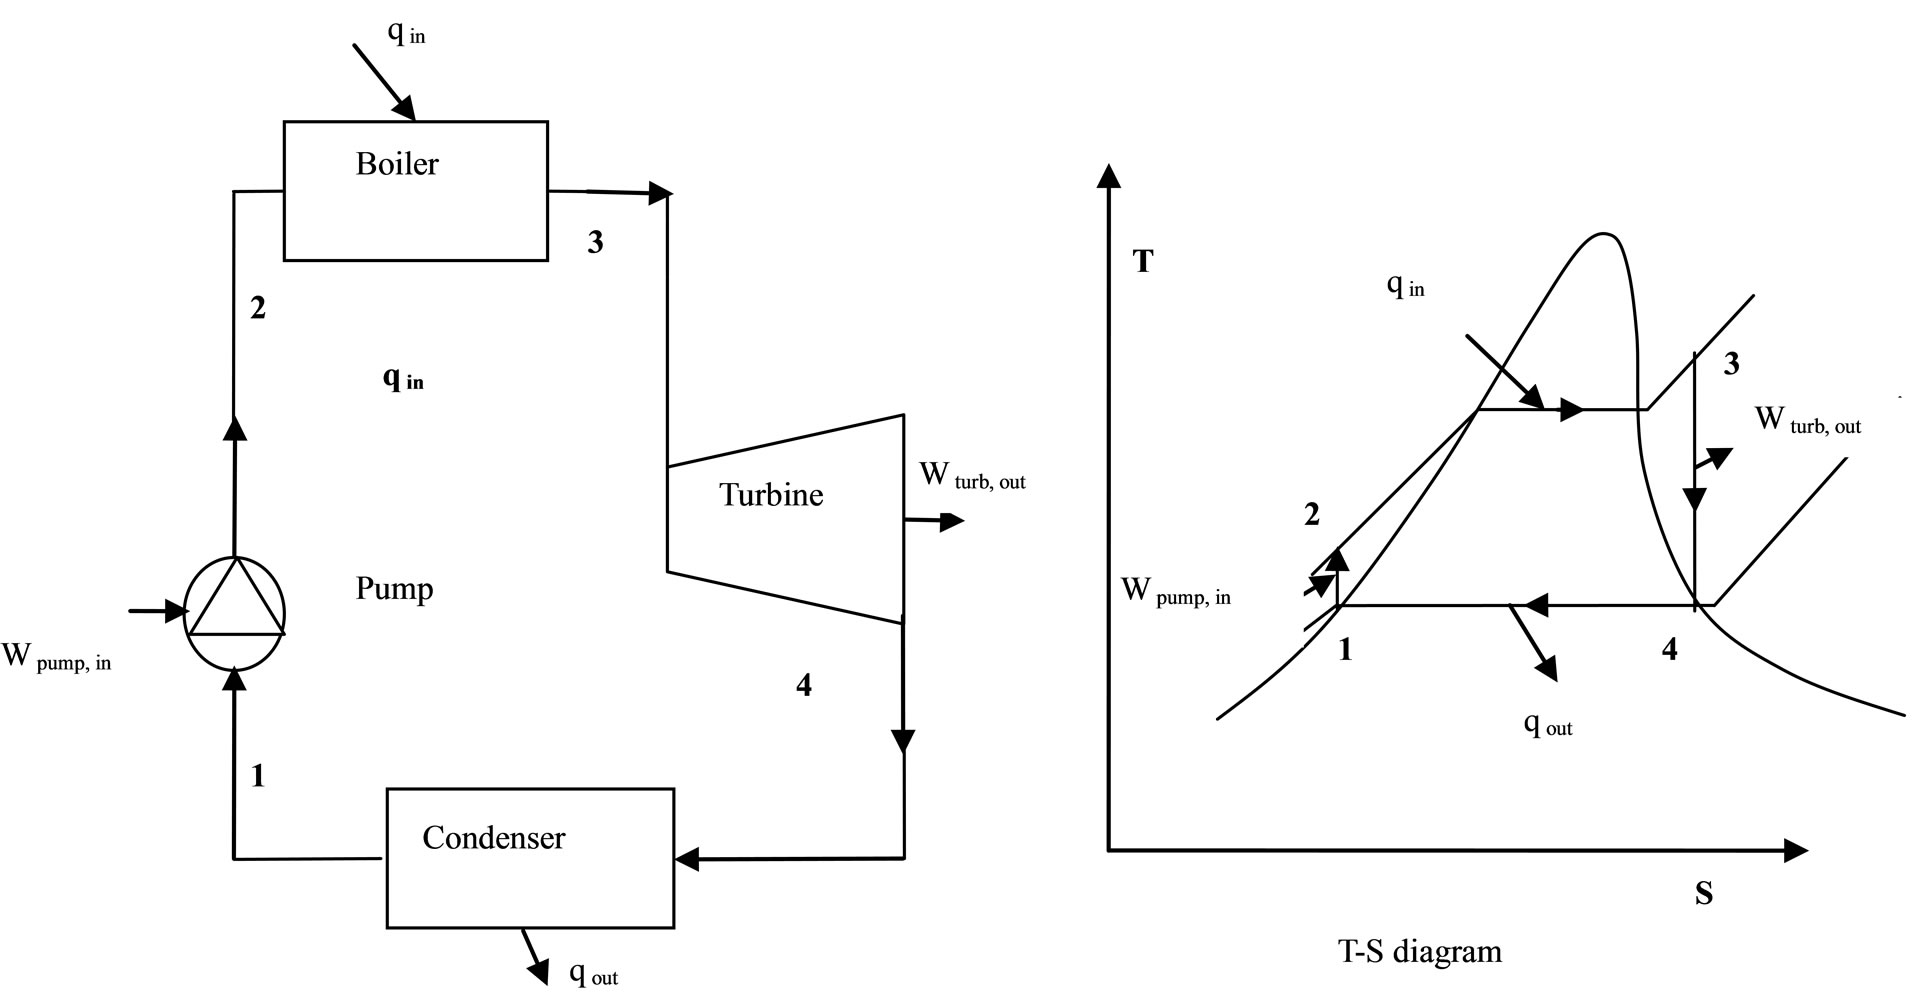
\includegraphics[width=\textwidth]{figures/review/rankine_steam.jpg}
  \caption{Steam Rankine cycle T-s diagram and physical layout\label{fig:rankine_steam} }
\end{figure}

The process is composed by four consecutive processes, as shown in Figure~\ref{fig:rankine_steam}:

\begin{itemize}
  \item \textbf{Process 1-2:} the working fluid is pumped from low to high pressure. Since the fluid is in liquid form, the work required for pumping is small.
  \item \textbf{Process 2-3:} the liquid at high pressure is heated at almost constant pressure by an external source until it becomes dry saturated vapor.
  \item \textbf{Process 3-4:} the dry saturated vapor is expanded through a turbine, hence generating power. The working fluid experience a decrease of pressure and temperature, with possible partial condensation.
  \item \textbf{Process 4-1:} the wet vapor enters the condenser and returns to saturated liquid conditions.
\end{itemize}



\subsection{Organic Rankine cycle}

The Organic Rankine Cycle (ORC) is a particular use case of a Rankine thermodynamic cycle. It's named for its use of an organic, high molecular mass fluid with a liquid-vapor phase change, or boiling point, occurring at a lower temperature than the water-steam phase change. The fluid allows Rankine cycle heat recovery from lower temperature sources such as coolant from internal combustion engines. The low-grade waste heat is converted into useful work, that can itself be converted into mechanical or electrical power. In Figure~\ref{fig:orc_diagram}, the T-s diagram and the plant layout for a generic Organic Rankine Cycle are shown. The formulation of the efficiency is the same as the Steam Rankine Cycle, shown in Equation~\ref{eq:eta_rankine}.

\begin{figure}[ht]
  \centering
  \includegraphics[width=0.8\textwidth]{figures/review/orc.jpg}
  \caption{T-s diagram and plant layout for a generic Organic Rankine Cycle\label{fig:orc_diagram} }
\end{figure}

The system itself is made of four components: evaporator, expander, condenser and pump. Usually a recuperator is also used, to increase the efficiency and hence the production of useful power. The waste heat is used in the evaporator to vaporize the working fluid and convert the heat in mechanical work in the expander.

The selection of the working fluid is of key importance in low temperature Rankine Cycles. Because of the low temperature, heat transfer inefficiencies have a major importance. In order to recover low-grade heat, the fluid generally has a lower boiling temperature than water, then refrigerants and hydrocarbons are two commonly used components. Water is a preferable working fluid for high exhaust gas temperatures ranging from \SI{500}{\celsius} to \SI{800}{\celsius}, while refrigerants are better suited fro lower temperatures, as in the gas of the exhaust gases. Water also has the disadvantage that requires superheating to avoid turbine blade erosion, but the high degree of superheating makes it less practical for automotive application due to the variation of exhaust temperature at different load conditions. In figure~\ref{fig:orc_working_fluids} are reported the different T-s diagram related to different Rankine cycle working fluids.

\begin{figure}[ht]
  \centering
  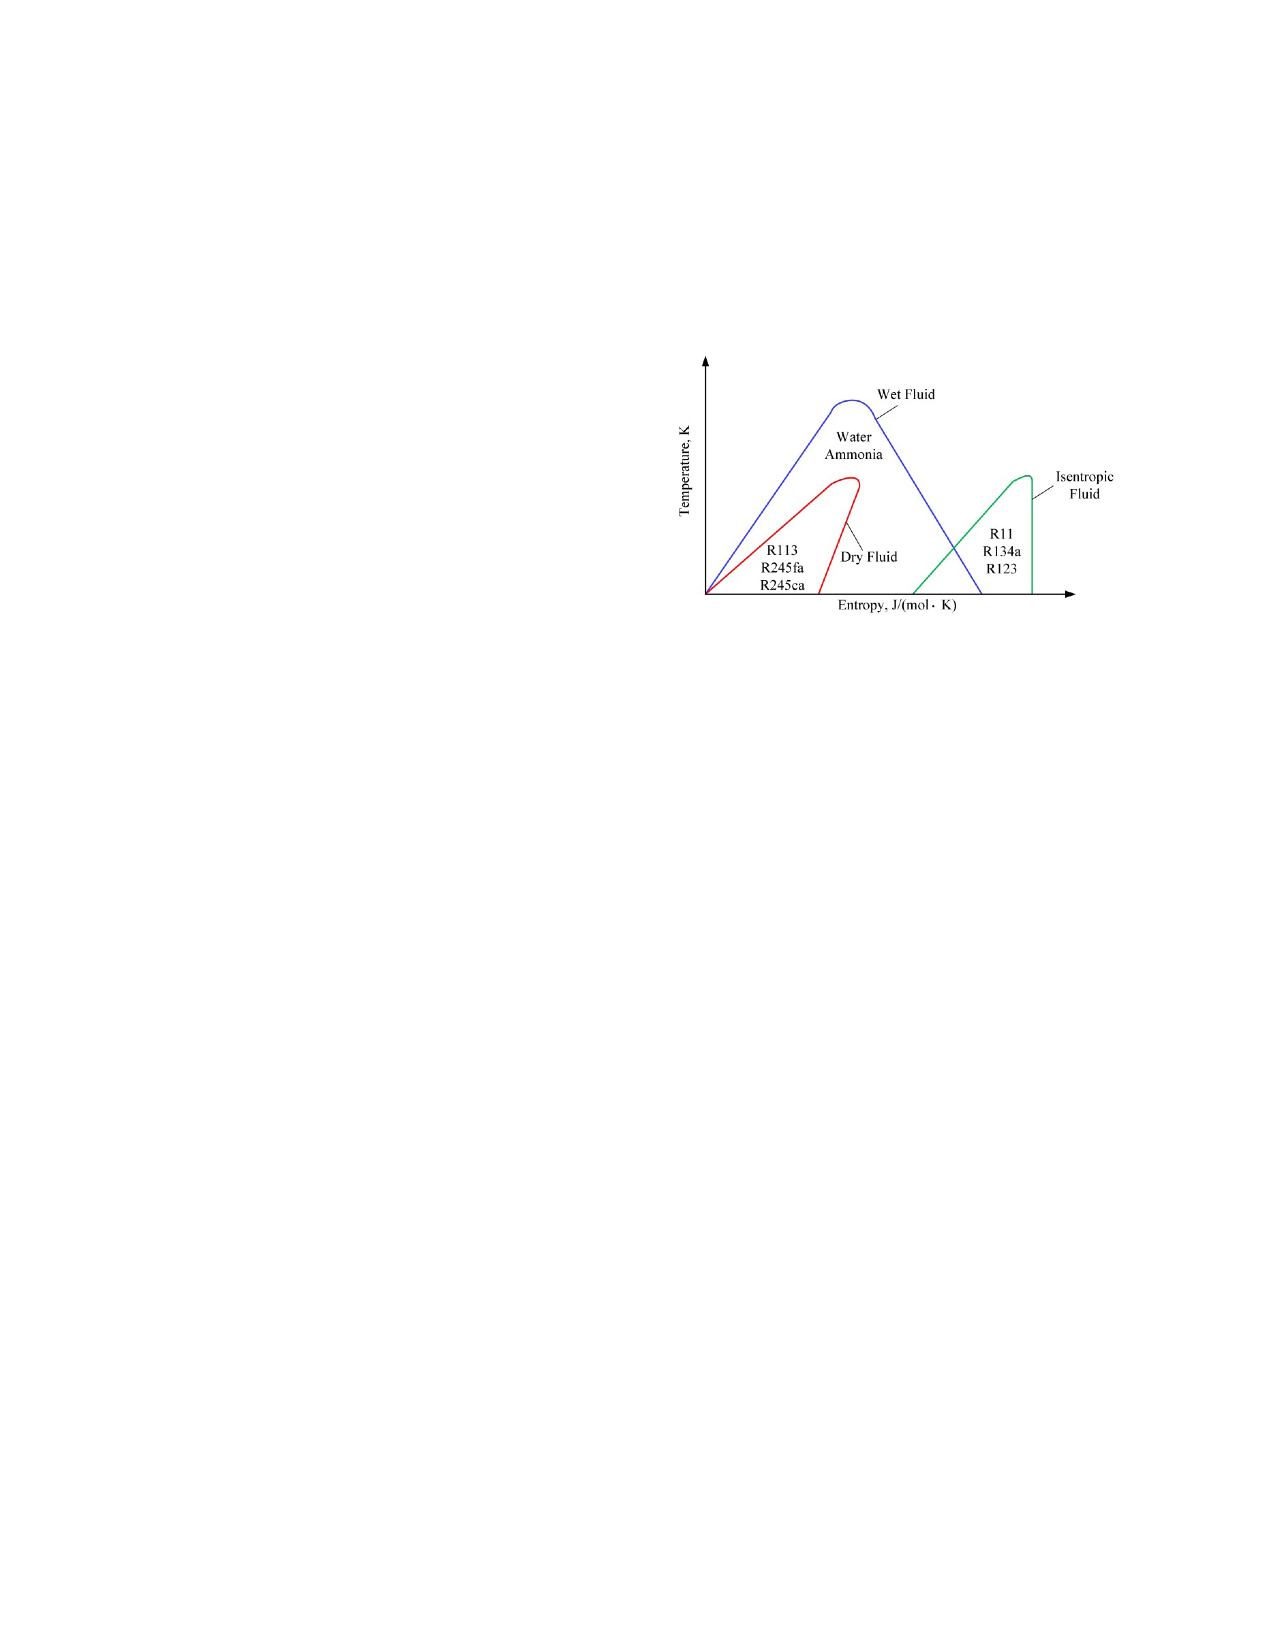
\includegraphics[width=0.7\textwidth]{figures/review/orc_working_fluids.pdf}
  \caption{Comparison of different Rankine Cycle working fluid characteristics\label{fig:orc_working_fluids} }
\end{figure}

In current years, an increasing environmental awareness has provoked the shifting from traditional refrigerants (i.e. R134a, R236fa, R245fa) to new refrigerants, characterized by lower harm potential to passengers in case of leakage or crashes, and a lower flammability level (i.e. R1233zd, R1234yf).

When considering an ORC coupled with an internal combustion engine, different possible configurations must be considered. The most common and simple structure utilizes the exhaust gas as the only heat source to evaporate the working fluid. The second structure adds another heat exchanger (recuperator) before the evaporator, using the steam from the expander to preheat the working fluid. A third structure uses waste heat from engine coolant to preheat the working fluid. The regenerative preheating of structure 2 requires a very complex liquid-gas heat exchanger with high exchange surfaces, while the preheater in structure 3 only requires a simple liquid-liquid heat exchanger. There have been contradicting conclusions about the effect of preheating using engine coolant on the RC system efficiency. Based on Vaja and Gambarotta's work \cite{Vaja2010}, the RC system with a preheater allows a net increase in power output, compared to structure 1, of 10\% to 35\%, depending on which working fluid is chosen. Alberto Boretti \cite{Boretti2012} also showed a 8.2\% fuel economy improvement using engine coolant to preheat the RC cycle, compared to a 6.4\% improvement when only exhaust gas is used to boil the working fluid. Arias et al. \cite{Arias2006} also compared the combined exhaust and engine coolant heat recovery system with the exhaust only structure. It was found that the additional power recovered from the engine coolant system was 20 W out of a total 2140 W, which is around 1\% improvement.

\begin{figure}[ht]
  \centering
  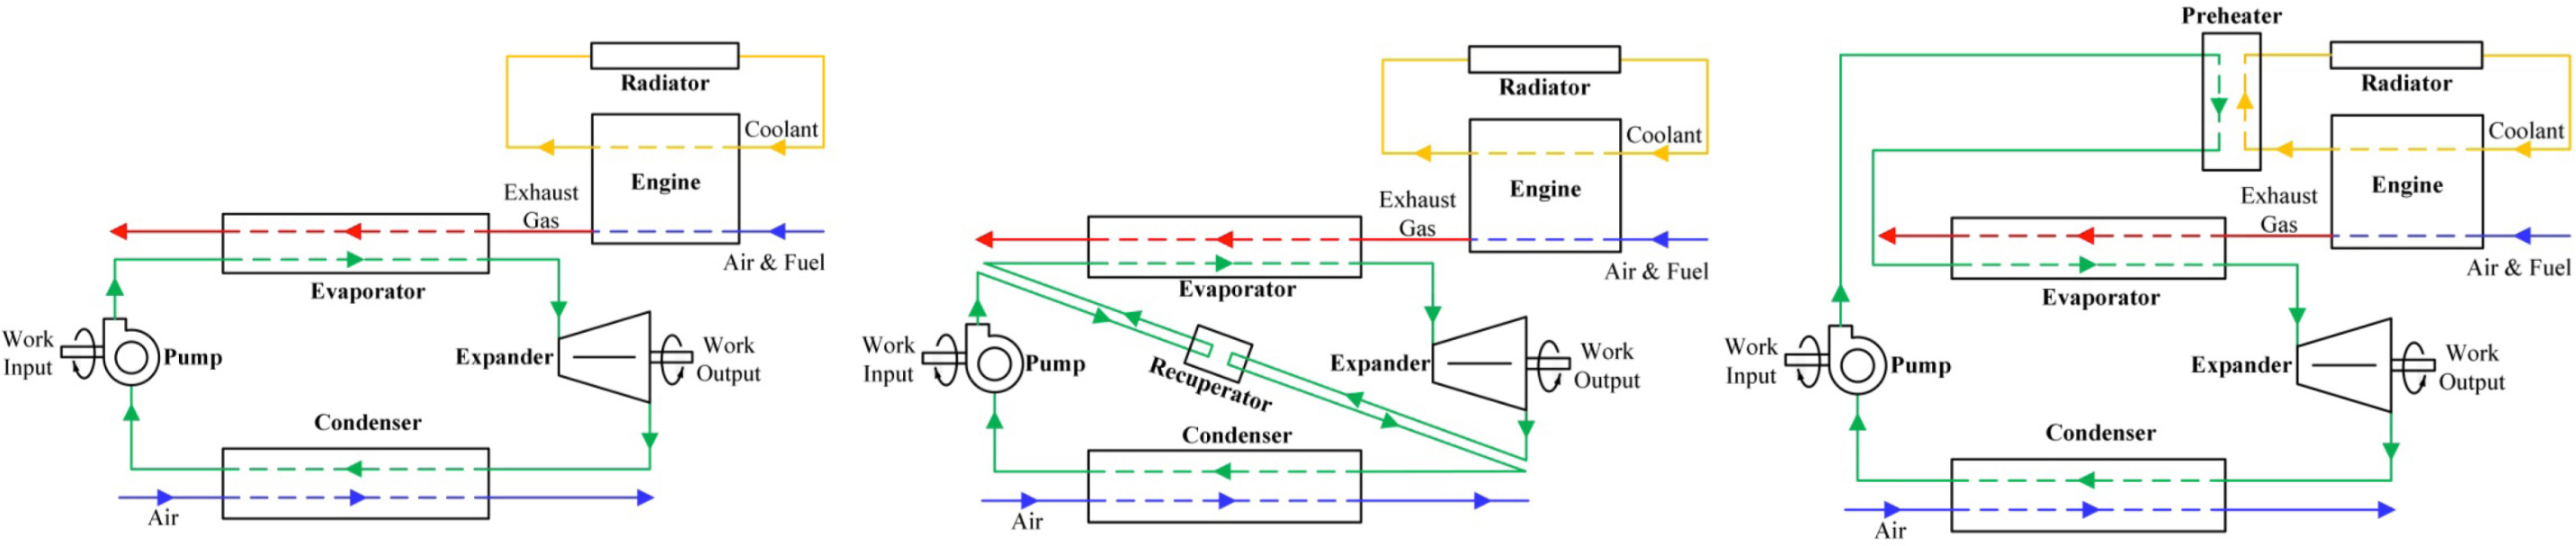
\includegraphics[width=\textwidth]{figures/review/orc_layouts.jpg}
  \caption{Different ORC layouts: structure 1, 2 and 3\label{fig:orc_layouts} }
\end{figure}

When selecting the different configurations, different factors have to be take into consideration as the maximization of the recovered energy is not the only objective to pursue. System complexity, component volume and weight, and the resulted extra cost added to the vehicles and the payback period are also big concerns.

\subsection{Brayton cycle}

The Brayton cycle is a thermodynamic cycle that uses a gas as a working fluid. The generalized plant configuration and the p-V and T-s diagrams are showed in Figure~\ref{fig:brayton_cycle}.

\begin{figure}[ht]
  \centering
  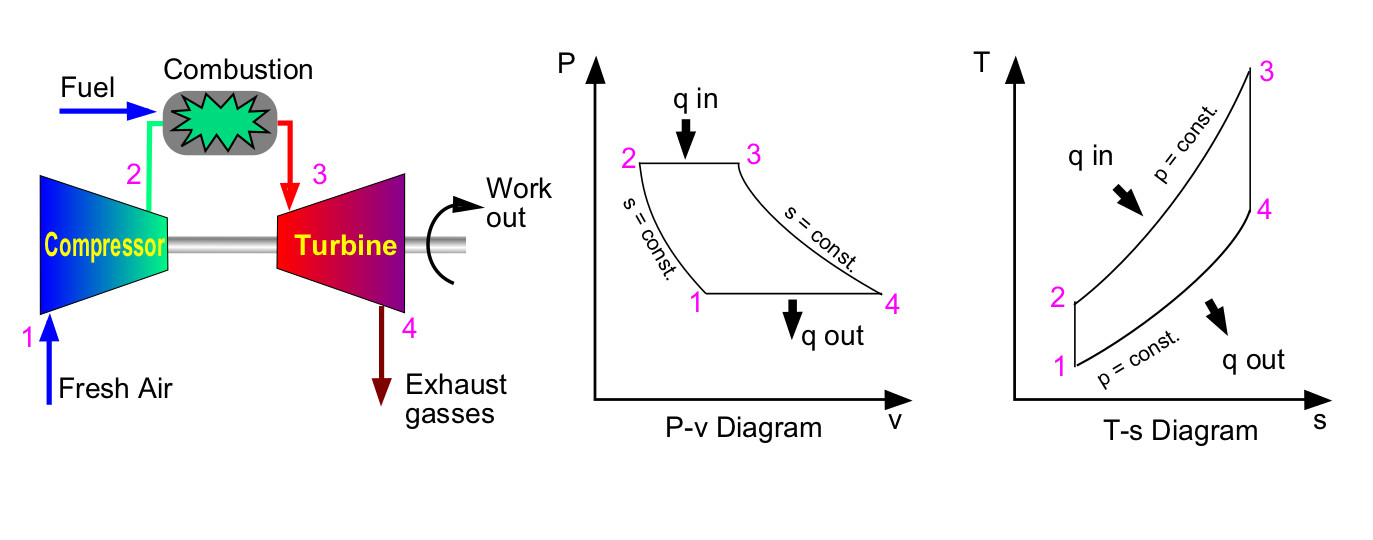
\includegraphics[width=\textwidth]{figures/review/brayton_cycle.jpg}
  \caption{Diagrams and plant layout of an idealized Brayton cycle\label{fig:brayton_cycle} }
\end{figure}

The cycle is composed by:

\begin{itemize}
\item \textbf{Process 1-2:} adiabatic compression, operated in a turbo-machine (compressor)
\item \textbf{Process 2-3:} isobaric heat addition, operated in the combustor
\item \textbf{Process 3-4:} adiabatic expansion, operated in a turbo-machine (turbine)
\item \textbf{Process 4-1:} isobaric heat rejection, operated in a radiator in the case of a closed cycle
\end{itemize}

The efficiency of the cycle can be calculated as:

\begin{equation}
  \eta_{t}=1-\frac{1}{\beta^{k-1}}
\end{equation}

The regular Brayton thermodynamic cycle proved itself not to be suited for a bottoming cycle type of application. Of particular importance for waste heat recovery applications is the \emph{Super-critical CO\textsubscript{2}} (sC02) Brayton cycle. Researchers claim \cite{Kimzey2012} that an sCO2 power cycle could potentially exhibit a higher thermal efficiency than steam cycles when operating between the same maximum and minimum cycle temperatures. In addition, the high energy density of sCO2 suggests that the size requirements for the turbomachinery used in an sCO2 power cycle could potentially be much lower than those used in steam cycle generation, which may result in lower capital costs. To date, most research in the field has been dedicated to the use of sCO2 as the primary power cycle in nuclear applications, but relatively little research has been aimed toward developing an sCO2 cycle that is well-suited to bottoming cycle applications.

\subsection{Selection of the bottoming cycle}

After having introduced the three most common thermodynamic cycles that can be employed as bottoming cycle, it's necessary to understand the up and downsides of the three in order to select the better one for the use case considered in this thesis.

The choice between the two different Rankine Cycles is basically reduces to the selection of the most appropriate working fluid. The choice of the working fluid to be used in the cycle depends on a number of factors, e.g thermodynamic efficiency, environmental protection, safety, process-related and economic issues.

The steam Rankine cycle is the most reliable and simple configuration considered, it has a high efficiency due to the very small work required for the pump. Water is widely available, cheap and does not present any issue in form of toxicity or environmental harm potential. The biggest downside of the selection of water is the huge latent heat of vaporization. According to Arias at al. \cite{Arias2006}, water is not suited to recover heat when used as a working fluid because of the mismatch between the low temperature of engine coolant and high boiling temperature of water. Water has been used in the fist generation of BMW's Rankine system \cite{Freymann2008} , the \emph{Turbosteamer}, to harvest energy from exhaust gases, while ethanol was used in a separate loop for engine coolant waste heat recovery. In the second generation Turbosteamer \cite{Freymann2012}, water is only been heated by the exhaust gases. This is because water works best when used for high exhaust gas temperature, from \SI{500}{\celsius} to \SI{800}{\celsius}. Water required also superheating to avoid turbine blade erosion, if turbine is selected as expander, but the high degree of superheating makes it less practical for the automotive application due to the variation of exhaust temperature at different load conditions. Besides, its high freezing point (\SI{0}{\celsius}) cannot meet the standard automotive working temperature range (\SI{-40}{\celsius} to \SI{85}{\celsius}).

Organic Rankine Cycle shows a much better potential for waste heat recovery in automotive applications. The low boiling point of the organic fluid allows to recover efficiently low-grade waste heat. The dry/isentropic refrigerants are widely used in small-scale RC applications because of their good heat transfer properties, excellent thermal stability and low viscosity. They are generally non-flammable, which is a big advantage for automotive application and compatible with most materials. Under typical low temperature ambient conditions they do not freeze, which is a major concern with water. Chammas and Clodic \cite{ElChammas2005} compared different organic fluids with water for RC application to hybrid vehicles, arguing that using water to recover automotive waste heat could lead to a complex system requiring large size equipment and high investment cost, which makes the study on organic working fluid necessary. Domingues et al. \cite{Domingues2012} compared R123 and R245fa with water as working fluid for vehicle RC waste heat recovery potential from exhaust gas. The study revealed the advantage of using water as working fluid to recover waste heat from exhaust gas of vehicles equipped with spark-ignition engine. However, it was also found that the heat exchanger effectiveness for R123 and R245fa is higher than that for water. Consequently, when the exhaust temperature is relatively low, organic fluids can be considered appropriate for vehicle RC application. Extensive work has also been poured in ORC + internal combustion engines combinations, leading to interesting fuel saving values.

The usage of organic fluids, such as refrigerants (i.e. R134a, R245fa, etc.) carries a few shortcomings. First, the intrisic property of dry/isentropic fluids reduce the area of net work in the T-s diagram, which means less power output compared to wet fluid, e.g. water. Second, to reduce the cooling load of the condenser, a recuperator is usually necessary to cool the superheated vapor to saturated state, increasing the system complexity and cost. Moreover, most organic fluids have relatively low thermal instability temperatures compared to water, therefore at high temperature and pressure the system might suffer chemical decomposition and deterioration. In addition, the current generation of refrigerants has a high global warming potential, which means that their use could be limited or banned in the near future.

The super-critical C0\textsubscript{2} Brayton cycle combines the advantages of both steam Rankine cycle and gas turbine system. In other words, the fluid is compressed in the incompressible region, and the higher turbine inlet temperature can be utilized with less material issues compared with the steam Rankine cycle. Therefore, the volumetric flow rate decreases as the fluid density is higher, resulting in 10 times smaller turbomachinery compared with the turbomachinery of a steam Rankine cycle \cite{Ahn2015}. In addition, researchers claim \cite{Kimzey2012} that an sCO2 cycle could potentially exhibit a higher thermal efficiency than steam cycle, when operating between the same maximum and minimum temperatures. A modeling research performed by Kimzey \cite{Kimzey2012} highlighted that the Brayton cycles are well suited to operating with a heat flux producing power source, but are not well suited to a sensible heat source, such as topping cycle exhaust. This is because this cycle is not truly effective at recovering waste heat: most Brayton cycles are not self-sustaining at operating temperatures below \SI{480}{\celsius}, a problem that revealed itself also in solar thermal plants. 

Given the above reasons, in this thesis an Organic Rankine Cycle has been selected as bottoming cycle to be modeled and coupled with the 3.6L V6 petrol engine Simulink model.

\section{Introduction to split cycle engines}

\subsection{Basic principles}

\subsection{A different approach to waste heat recovery: integrated WHR}.
